\documentclass{ctexart}
\pagestyle{plain}
\usepackage{makecell,rotating,multirow,diagbox,booktabs,caption}
\usepackage{indentfirst}
\usepackage{tabularx}
\usepackage{amsmath}
\usepackage{graphicx}
\usepackage{color}
\usepackage{geometry}
\date{}


\title{\begin{huge} \textbf{APP拍照任务的定价}  \end{huge}}


\begin{document}
\maketitle


\begin{large}
\textbf{摘要}

本文建立APP拍照任务的定价模型和算法。

对于问题一,以每一个任务为主体,提取该任务的位置,周边会员的位置,预选时间,预选额度以及信誉度信息,将已给的定价视为精准定价,进行线性回归,得出一组系数最优解。为了定性分析任务失败的原因,定义实际和理论定价的差值与理论定价的比值为增值比,进一步根据增值比对任务分类,用每类任务增值比的平均值作为任务能否完成的阈值,借此来给出任务失败的原因。

对于问题二,我们试着从多个角度来回答。角度一是利用上一问中求出的阈值,将任务增值比与其比较,对成功的且价格过高的任务,提取出多余的价格,对失败的且价格偏低的任务,增补欠缺的价格,以此实现价格优化;角度二是优化问题一的模型,考虑变量之间的相互影响,重新回归,得出新的理论价值;角度三是利用任务完成情况确定不等式,采用线性规划的知识确定出系数最优解。

对于问题三,经过分析,采用外围收缩技术,每次利用重心转移法选取最外围的点,从该点开始打包,逐步向内部收缩。打包完成后,将每一个任务包视为一个主体,重新确立回归方程,进行线性回归,求出最优解。之后结合前两问,选取评判任务包完成与否的标准,最后统计任务包完成数目,与之前的结果相比较。

对于问题四,先使用第三问的方法,对任务进行分类打包,然后利用问题三中拟合的线性模型对每个任务包定价。



\textbf{关键字:}
线性回归\ \ 阈值比较\ \ 外围收缩\ \ 重心转移法
\end{large}
\newpage
 \section{\leftline{问题重述}}
“拍照赚钱”是移动互联网飞速发展下,应运而生的一种新型自助式服务模式。用户成为APP的会员后,从APP上领取需要拍照的任务,赚取APP对任务所标定的酬金。这种基于移动互联网的自助式劳务众包平台,为企业提供各种商业检查和信息搜集,相比传统的市场调查方式可以大大节省调查成本,而且有效地保证了调查数据真实性,缩短了调查的周期。因此APP 成为该平台运行的核心,而APP中的任务定价又是其核心要素。如果定价过高,将导致投资成本的浪费;如果定价过低,有的任务就会无人问津,而导致商品检查的失败。请讨论以下问题:

\textcircled{\small{1}} 根据已给的信息,包括任务的位置,完成情况,会员的位置,预选时间,预选限额,信誉度,探索定价的规律。

\textcircled{\small{2}}优化定价方案,重新给出定价,并与原方案比较。


\textcircled{\small{3}}考虑如何将任务分类聚合,打包分派,以避免恶性竞争,提高运行效率。

\textcircled{\small{4}}根据以上的模型,对于新一批的任务,给出定价。



\section{\leftline{问题分析}}
定价策略,市场营销组合中一个十分关键的组成部分。价格通常是影响交易成败的重要因素,同时又是市场营销组合中最难以确定的因素。由此可见定价问题本身就具有一定的难度。而这种新型的自助服务运营模式又有别于以往的定价模型。在问题当中,会员是信息的提供者,即通常意义下的生厂商,而APP平台花钱买信息,是消费者。所以在拍照任务定价中,是消费者定价,来吸引生产者,与以往的定价形式有很大的不同,这也正说明了拍照任务定价本身具有一定的特殊性。

给任务定价时通过对任务以及会员信息的筛选,整合,提取,拟合来实现对任务定价规律的探索,从而在此基础上优化定价,包括以下三个步骤:

(1)任务和会员信息的预处理,包括数据清洗,数据分类,数据整合;

(2)任务定价规律的探索,应用适当的回归算法找出任务定价与其他信息之间的关系;

(3)优化任务定价模型,给出更为合理的定价;


(4)运用已经得到的模型,给新一批的任务定价。

其中步骤(2)(3)是算法实现的核心,直接关系到任务定价的合理性,从而影响任务的完成与否。

\section{\leftline{模型假设}}

(1)假设会员的任务预定时间只是会员获取任务时竞争力的衡量指标,而不去考察具体的时间分配;

(2)假设会员的任务限额只是会员获取任务时竞争力的衡量指标,而不去考察会员具体获得多少任务;

(3)假设任务一经会员领取就会被执行,即视为成功的任务。
\section{\leftline{符号说明}}

\begin{table}[h]\centering\footnotesize
\begin{tabular}{c c }
\bottomrule[1pt] 
 符号&描述\\

\hline
$r^{j}_{i}$&第i个任务的经度\\
$r^{w}_{i}$&第i个任务的纬度\\
$\overline{r^{j}}$&任务的平均经度\\
$\overline{r^{w}}$&任务的平均纬度\\
$R^{j}_{i}$	&第i个任务包的经度\\
$R^{w}_{i}$&第i个任务包的纬度\\
$(\overline{r^{j}},\overline{r^{w}})$&任务的重心位置\\
$h^{j}_{i}$&第i个会员的经度\\
$h^{w}_{i}$&第i个会员的纬度\\
$\overline{h^{j}}$&会员的平均经度\\
$\overline{h^{w}}$&会员的平均纬度\\
$(\overline{h^{j}},\overline{h^{w}})$&会员的重心位置\\
$t_{i}$&第i个会员的时间\\
$e_{i}$&第i个会员的限额\\
$x_{i}$&第i个会员的信誉\\
$v_{i}^{s}$&第i个任务的实际定价\\
$v_{i}^{l}$&第i个任务的理论定价\\
$V^{s}_{i}$	&第i个任务包的实际价格\\
$V^{l}_{i}$	&第i个任务包的理论价格\\
$d_{i}$&第i个任务的增值比=(实际价格-理论价格)/理论价格\\
$D_{i}$&	第i个任务包的增值比=(任务包实际价格-理论价格)/理论价格\\
$m_{h}$&平均任务竞争会员数=会员预定总限额/任务总数\\
$m_{r}$&平均竞争任务数=会员预定总限额/会员总数\\
$b_{\uppercase\expandafter{\romannumeral1}}$&第一类任务($d_{i}>0$,完成)的平均增值比\\
$b_{\uppercase\expandafter{\romannumeral2}}$&第二类任务($d_{i}>0$,失败)的平均增值比\\
$b_{\uppercase\expandafter{\romannumeral3}}$&第三类任务($d_{i}<0$,完成)的平均增值比\\
$b_{\uppercase\expandafter{\romannumeral4}}$&第四类任务($d_{i}<0$,失败)的平均增值比\\
\bottomrule[1pt] 
\end{tabular}
\end{table}





\section{\leftline{模型的建立和求解}}
\subsection{问题1分析}

该问要求我们探索任务定价规律。参考附件一,附件二所给信息,我们可知,可能和定价相关的变量有任务的位置,会员的位置,预选限额,预先时间以及信誉度。根据金融经济学中的线性定价法则[1]我们假设任务价格和所涉及的变量成线性关系。之后我们选取任务理论价格和实际价格之差的绝对值之和(以下简称绝对值和)作为量度标准,也即绝对值和越小,匹配度越高,模型越发吻合实际。利用线性回归求解出匹配度最高的解。并且根据相关类似模型[2]可知,会员和任务的相对距离越远,会员的信誉度越高,预定限额越大,预定时间越短,会员执行任务所需的酬金越高。得出最优解后,需判断是否符合上述规律。接着我们定义增值比=(实际价格-理论价格)/理论价格,用以判断和度量任务实际定价相比于理论定价的变化情况,并以此来求出任务完成或失败的阈值,进而定量地分析任务失败的原因

1)问题1的模型建立与求解

问题1要求对于附件一中的任务探索其定价规律。本文通过以下几个步骤建立模型

步骤一:首先进行数据清洗,使用统计学的方法,即正态分布$3\sigma$原则,对任务的位置,会员的位置,预选限额,预先时间以及信誉度进行正态拟合,剔除边缘数据。以会员的位置为例:

 \ \ \ \ \ \ \ \ \ \ \ \  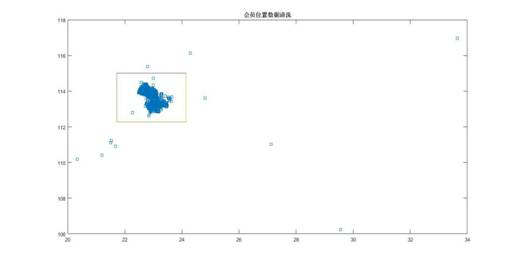
\includegraphics[width=10cm]{1.jpg}


 然后根据任务和会员的位置信息,利用MATLAB画出其分布图,并分别求出其重心;

\ \ \ \  \ \ \ \ \ \ \ \ \ 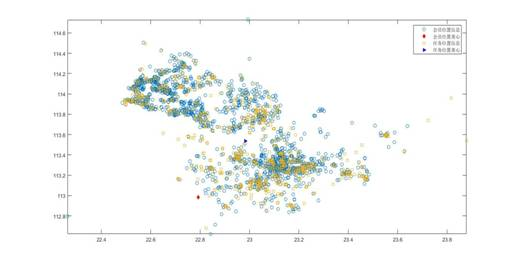
\includegraphics[width=10cm]{2.jpg}


步骤二:我们作如下定义:平均任务竞争会员数$m_{h}$=会员预定总限额/任务总数,平均任务竞争会员数的含义是:每个任务平均有多少个会员去竞争。经计算可知,$m_{h}$=15,即每个任务有15名会员竞争。并且之前我们假设任务的定价与会员和任务的距离成线性关系,更加具体一点就是,会员和任务的距离越大,任务定价越高。当任务的定价无限增大,自然可以吸引所有的会员来竞争它,但是这显然是不合理的。所以我们需要让任务的定价尽可能小,但是又能够吸引一定的会员来竞争它。因此我们假设竞争每个任务的15个会员是最邻近该任务的15个人。具体操作如下:以每个任务为圆心,以不同的半径画圆,保证每个圆内的会员数为15,将圈内的会员成为与其竞争的会员。

 \  \ \ \ \ \ \ \ \ \ \ \ \ \ 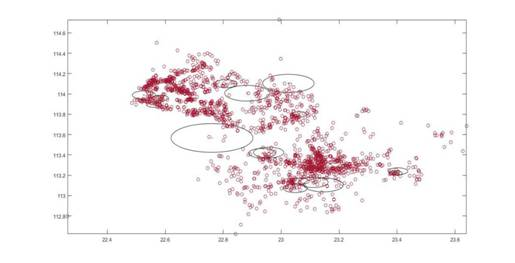
\includegraphics[width=10cm]{3.jpg}



步骤三:确定影响因素,可能对任务定价产生影响的变量有:任务位置到任务重心的距离$| r^{j}_{i} -\overline{r^{j}}|$,$|r^{w}_{i}-\overline{r^{w}}|$;竞争会员的位置到会员重心的距离$| h^{j}_{k} -\overline{h^{j}}|$,$|h^{w}_{k}-\overline{h^{w}}|$;
竞争会员到任务的距离$((h^{j}_{k}-r^{j}_{i})^{2}+(h^{w}_{k}-r^{w}_{i})^{2})^{\frac{1}{2}}$\; 以及竞争会员预定时间$t_{k}$,预定限额$e_{k}$以及信誉值$x_{k}$,假设所有变量与任务定价都是线性关系,即

$v^{l}_{i}=a^{j}|r^{j}_{i}-\overline{r^{j}}|+a^{w}|r^{w}_{i}-\overline{r^{w}}|$
$+\sum\limits_{k\in O}(q^{j}|h^{j}_{k}-\overline{h^{j}}|+q^{w}|h^{w}_{k}-\overline{h^{w}}|+x_{k}(p_{3}((h^{j}_{k}-r^{j}_{i})^{2}+(h^{w}_{k}-r^{w}_{i})^{2})^{\frac{1}{2}}+p_{1}t_{k}+p_{2}e_{k})+c$

问题划归为求解系数$a^{j},a^{w},q^{j},q^{w},p_{1},p_{2},p_{3} ,c$

步骤四:假设给出的任务定价均为精准定价,也即不考虑任务完成情况。选理论定价与实际定价差的绝对值之和作为衡量标准,采用线性回归,求解出最优系数。

    步骤五:对每个任务,定义增值比$d_{i}=(v^{s}_{i}-v^{l}_{i})/v^{l}_{i}$,根据拟合的结果,可以求出每个任务的增值比,之后用增值比来分析任务完成和失败的原因。




2)定价模型好坏的量度
系数选取的是否吻合,我们采用绝对差算法来刻画,数学描述如下:

$$ \sum^{N}_{k=1}|v^{s}_{k}-v^{l}_{k}|$$

$N$  表示任务总数

   $v^{s}_{i}$  表示第i个任务的实际定价

$v^{l}_{i}$   表示第i个任务的理论定价

3)模型求解

(1)利用线性回归求出系数最优解。

以任务$i$为例,与其定价$v^{l}_{i}$  有关的变量:$|r^{j}_{i} -\overline{r^{j}}|$,$|r^{w}_{i}-\overline{r^{w}}|$(任务的位置信息),$|h^{j}_{k}-\overline{h^{j}}|$,$|h^{w}_{k}-\overline{h^{w}|}$(竞争会员位置信息),$((h^{j}_{k}-r^{j}_{i})^{2}+(h^{w}_{k}-r^{w}_{i})^{2})^{\frac{1}{2}}$(竞争会员与任务的距离),$t_{k}$,$e_{k}$,$x_{k}$(竞争会员信息).

假设所有的变量成线性关系,也即


$v^{l}_{i}=a^{j}|r^{j}_{i}-\overline{r^{j}}|+a^{w}|r^{w}_{i}-\overline{r^{w}}|$
$+\sum\limits_{k\in O}(q^{j}|h^{j}_{k}-\overline{h^{j}}|+q^{w}|h^{w}_{k}-\overline{h^{w}}|+x_{k}(p_{3}((h^{j}_{k}-r^{j}_{i})^{2}+(h^{w}_{k}-r^{w}_{i})^{2})^{\frac{1}{2}}+p_{1}t_{k}+p_{2}e_{k})+c$


则我们的目标是选取系数$a^{j},a^{w},q^{j},q^{w},p_{1},p_{2},p_{3} ,c$,使得$ \sum\limits^{n}_{k=1}|v^{s}_{k}-v^{l}_{k}|$ 达到最小。

用MATLAB 求解结果如下:

$a^{w}= -1.258559895431065$

 $a^{j} =4.475039754284610$


$q^{j}=0$

           $q^{w}=0$


$p_{1} = -0.000847039018016$

$p_{2}=0.000000529712632$

 $p_{3}=0.006211717598381$

$c=68.079526475834584$

下面根据解的情况给出相应解释。首先可以看出,$a^{w}$为负数,即$|r^{w}_{i}-\overline{r^{w}}|$越大,定价就越低;而$a^{j}$为正数,即$|r^{j}_{i}-\overline{r^{j}}|$越大,定价就越高。而且$|a^{j}|>|a^{w}|$,也就是说经度变化带来的影响要比纬度的大。根据深圳市地形地貌,我们给出如下解释。

\
\begin{figure}
 \ \ \ \ \ \ \ \ \ \ \ \ \ \  \ \ \ \  \ \ \ \  \ \ \  \ \  \ \ \ 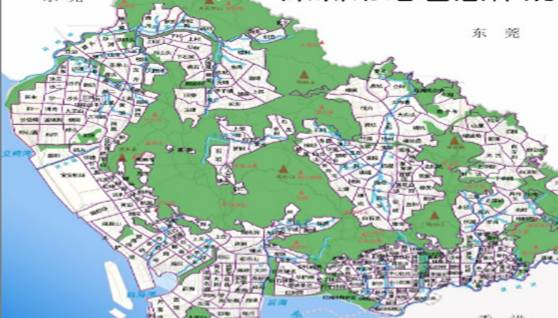
\includegraphics[width=7.5cm]{4.jpg}
\caption*{深圳市地图}
\end{figure}


\begin{figure}
  \ \ \ \ \ \ \  \ \ \ \ \ \ \  \ \ \ \  \  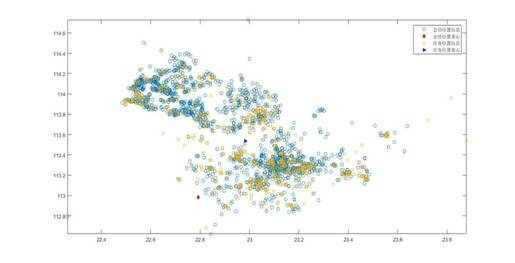
\includegraphics[width=10cm]{5.jpg}
   \caption*{任务分布图}
  \end{figure}

 从地图上可以看出,任务位置的分布与经济繁华地带的分布基本一致。
  深圳市繁华地段主要沿经线,呈东西条带状分布。因此我们可以根据纬度的差异将繁华地带分成若干个区域,每个区域近似看成沿着经线分布的狭长地带,在每个区域内任务位置沿着经线分布。对于会员而言,他们偏爱选择邻近的任务,也即是说,他们更加偏好选取和他们在一个区域内的任务,而不愿意跨区域去执行任务,因此,任务的定价与纬度呈负相关,所以$a^{w}$ 的符号为负。而在同一个区域内,会员可能选择任何一个任务去执行。对于远离重心的任务,相对来说比较偏远,只有给出的酬金更高,才能吸引会员去执行它,因此任务的定价与经度成正相关,所以$a^{j}$ 为正数。并且在繁华地带,正所谓寸土寸金,经度的微小变化,都会带来周边经济实力的巨大差异,所以
  $|a^{j}|$ 的数值较大。此外会员自身位置对于价格无影响,但是会员和任务的相对位置有影响,这和认知相符。并且从其他系数的正负可以看出,这组解与之前的假设:会员和任务的相对距离越远,会员的信誉度越高,预定限额越大,预定时间越短,会员执行任务所需的酬金越高,相符,所以我们可以认为这组解是可行的。并且从系数的大小可知,影响任务定价的主要是位置因素。

  (2)分析失败原因。

我们定义$d_{i}=(v^{s}_{i}-v^{l}_{i})/v^{l}_{i}$为任务$i$ 的增值比。由增值比的正负,我们可以看出任务的实际定价是高于还是低于理论定价;由增值比绝对值的大小,可以知道任务提价抑或降价幅度的大小。下面我们利用增值比将任务分为四种:

第\uppercase\expandafter{\romannumeral1} 类表示$d_{i}>0$,且任务完成;\ \ 第\uppercase\expandafter{\romannumeral2}类表示$d_{i}>0$,任务失败;

第\uppercase\expandafter{\romannumeral3}类表示$d_{i}<0$,但任务完成;
第\uppercase\expandafter{\romannumeral4}类表示$d_{i}<0$,任务失败。

将任务分类完成后,我们分别计算每一类中任务增值比的平均值,分别记为$b_{\uppercase\expandafter{\romannumeral1}}$,$b_{\uppercase\expandafter{\romannumeral2}}$,$b_{\uppercase\expandafter{\romannumeral3}}$,$b_{\uppercase\expandafter{\romannumeral4}}$。MATLAB
计算结果如下:

\begin{table}[!h]\center
\begin{tabular}{|c|c|c|c|}
\hline
第\uppercase\expandafter{\romannumeral1} 类&第\uppercase\expandafter{\romannumeral2} 类&第\uppercase\expandafter{\romannumeral3} 类&第\uppercase\expandafter{\romannumeral4} 类\\
\hline
$b_{\uppercase\expandafter{\romannumeral1}}$=0.06546& $b_{\uppercase\expandafter{\romannumeral2}}$=0.04972& $b_{\uppercase\expandafter{\romannumeral3}}$=-0.03433& $b_{\uppercase\expandafter{\romannumeral4}}$=-0.04393\\
\hline
\end{tabular}
\end{table}













由此可见$b_{\uppercase\expandafter{\romannumeral1}}$>$b_{\uppercase\expandafter{\romannumeral2}}$,$b_{\uppercase\expandafter{\romannumeral3}}$>$b_{\uppercase\expandafter{\romannumeral4}}$。所以对于失败的任务可做如下的解释:对于第\uppercase\expandafter{\romannumeral2}类的任务,虽然增值比大于零,即实际定价高于理论定价,但是由于它们价格的增幅还不够大,竞争力不够强,还不足以吸引会员来领取它,所以导致失败。而第\uppercase\expandafter{\romannumeral4}类的任务,增值比小于零,即实际定价低于理论定价,并且相比于同样降价的任务,降价幅度过大,让会员无法接受,所以任务失败。(如表1,表2所示)

除了上述的失败原因分析,我们还能做更深入的思考:对于第\uppercase\expandafter{\romannumeral2}类的任务,他们失败的原因是价格增幅还不够大,所以我们可以把$b_{\uppercase\expandafter{\romannumeral1}}$作为一个阈值,当这些任务的价格增值比达到$b_{\uppercase\expandafter{\romannumeral1}}$时,即可认为第
\uppercase\expandafter{\romannumeral2}类的任务由原来的失败变为了成功,同样的$b_{\uppercase\expandafter{\romannumeral3}}$可以作为第
\uppercase\expandafter{\romannumeral4}类任务的阈值。我们可基于这样的思考,对它们的价格进行调整,具体做法将在第二问详述。




\begin{table}[!h]\center\scriptsize
\begin{tabular}{|c|c|c|c|c|c|}
\hline

任务号码&	任务gps 纬度	&任务gps经度	&任务标价	&任务执行情况	&增值比\\
\hline
A0398&	23.37803295&	113.2569259&	75	&1	&0.068797\\
\hline
A0400&	23.40329889	&113.2398514	&75	&1	&0.067734\\
\hline
A0225&	23.33887144&	113.1110649	&75&	1	&0.067394\\
\hline
A0393&	23.446661	&113.2201755	&75	&1	&0.065477\\
\hline
A0157&	23.14872294	&113.5152914	&73.5	&0	&0.053621\\
\hline
A0169&	23.38627895	&113.410599	&74	&0	&0.049487\\
\hline
A0446&	22.68155741&	113.9462038&	72&	0	&0.048663\\
\hline
A0596&	22.94081692&	113.0626781	&72.5	&0	&0.048107\\
\hline


\end{tabular}
\end{table}
\ \ \ \ \ \ \ \ \ \ \ \ \ \ \ \ \ \ \ \ \ \ \ \ \ \ \ \ \ \ \ \ \ \ $d_{i}>0$时任务完成情况的对比
\newpage

  \begin{table}[!h]\center\scriptsize
\begin{tabular}{|c|c|c|c|c|c|}
\hline

任务号码&	任务gps 纬度&	任务gps经度	&任务标价	&任务执行情况	&增值比\\
\hline
A0615&	22.97994563&	114.0020847&	67&	1&	-0.033637\\
\hline
A0034&	22.5829933&	114.1471227&	66&	1&	-0.034192\\
\hline
A0534&	22.99313225&	113.7323716&	67&	1&	-0.034231\\
\hline
A0759&	23.04235254&	113.7318371&	67&	1&	-0.034912\\
\hline
A0095&	22.60766979&	113.8685312&	65.5&	0&	-0.044379\\
\hline
A0118&	22.607611&	113.8698943&	65.5&	0&	-0.044489\\
\hline
A0608&	23.01281035&	113.1202326&	66&	0&	-0.045097\\
\hline
A0391&	23.13562043&	113.3048107&	65&	0&	-0.045216\\
\hline



\end{tabular}


\end{table}
\ \ \ \ \ \ \ \ \ \ \ \ \ \ \ \ \ \ \ \ \ \ \ \ \ \ \ \ \ \ \ \ \ \ $d_{i}<0$时任务完成情况的对比

\begin{figure}[!h]\centering
\ \ \ \ \ \ \ \ \  \ 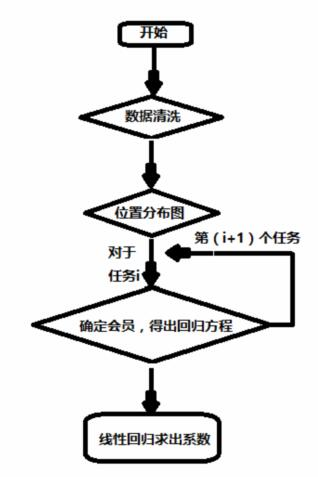
\includegraphics[width=8cm]{流程图1.jpg}
\caption*{问题1流程图}
\end{figure}


\subsection{问题2分析}

该问题要求我们对于附件一中的项目设计新的定价方案,并与原方案相比较。此时便会面临两个难题:一是从表格一,我们可以看出按照表格一中的定价,并不是所有的任务都完成了。这说明,附件一中所给的定价,并不能视为阈值定价,只能看成是阈值定价的一个估计限,因此我们需要找出一个阈值定价,当定价$\geq$阈值,任务完成,$\leq$阈值,任务失败,以此来判断定价变化后,任务的完成情况;二是存在一些与认知相不符的情况,比如定价比理论值高,但是仍失败,定价比理论值低,却成功。所以这促使我们对任务进行聚类处理,考察局部性质。

针对存在的问题,便可以从多个角度来解答:第一个角度是在问题一当中,我们已经根据实际的定价拟合出了一个模型,此时能容易定义一个阈值定价,在此基础上对价格进行微调,提高任务完成率,这可视为一个新的定价方案;第二个角度是,对问题一中的模型进行改进。在问题一当中,我们将会员的预选限额,预选时间以及信誉度当成独立的变量,而在题目当中提到,信誉度越高,预选时间越长,预选限额也越大,所以我们可以考虑这三个量之间的相互关系,以此来优化模型,重新定价;第三个角度是不改变问题一中的模型,利用线性规划的知识重新选定系数,使其达到最优。


具体的分析如下。

\

\textbf{角度一:}根据问题一的结果微调价格
    由问题一最后的分析可以发现,第\uppercase\expandafter{\romannumeral2}类,第\uppercase\expandafter{\romannumeral4}类的任务是失败的任务,根据之前的解释,如果我们分别将$b_{\uppercase\expandafter{\romannumeral1}}$,$b_{\uppercase\expandafter{\romannumeral3}}$当成第
    \uppercase\expandafter{\romannumeral2}类,第\uppercase\expandafter{\romannumeral4}类的任务的阈值,则我们希望能够对这些失败任务的价格进行微调,使之达到阈值。相反的,对于第\uppercase\expandafter{\romannumeral1}类和第
    \uppercase\expandafter{\romannumeral3}类这些成功的任务,有些增值比大于$b_{\uppercase\expandafter{\romannumeral1}}$,$b_{\uppercase\expandafter{\romannumeral3}}$,说明这份多出的价格是多余的,所以我们希望在确保这些任务仍然能被完成的情况下,适当降低价格。但是如果我们贸然直接使用$b_{\uppercase\expandafter{\romannumeral1}}$ 和$b_{\uppercase\expandafter{\romannumeral3}}$ 去给任务重新定价,则会出现任务$i$属于第
    \uppercase\expandafter{\romannumeral1}类的任务,但是$d_{i}<0$,也即此时无法从这个成功完成的任务中拨出多余的价格。所以为了更加精细的分析,我们对于每个任务计算其局部阈值。

     1)局部范围大小的选取
我们定义:平均竞争任务数$m_{r}=$会员预定总限额/会员总数,平均竞争任务数的含义是多少个任务去竞争一个会员领取它。经matlab计算$m_{r}=7$,即7个任务去竞争一个会员领取它。从问题一中的回归模型可知,影响任务定价主要是位置因素,所以每个任务主要是和邻近的任务去竞争会员。所以我们在地图上以每个任务画圈,使得圈内的任务数为7,圈内的任务称为竞争任务。

\ \ \ \ \ \ \  \ \ \ \ \ \ \ \ \  \ \  \ \ \ \  \ 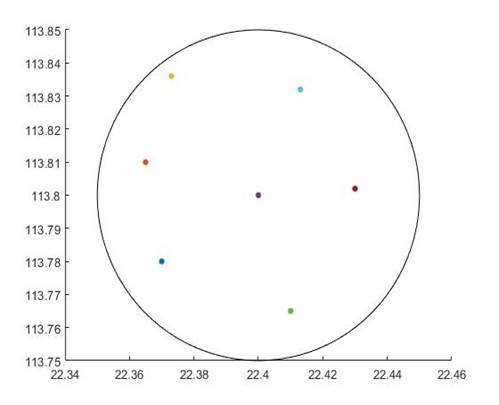
\includegraphics[width=7cm]{8.jpg}

2)局部阈值的确定
以任务$i$为例,对于圆圈$i$内的7个竞争任务,将其归为四类,即之前所说的第\uppercase\expandafter{\romannumeral1}类,第\uppercase\expandafter{\romannumeral2} 类,第\uppercase\expandafter{\romannumeral3}类,第\uppercase\expandafter{\romannumeral4}类。然后计算出这四类中的任务的增值比的平均值,将其作为任务$i$的局部阈值,记为$b_{\uppercase\expandafter{\romannumeral1}i}$,$b_{\uppercase\expandafter{\romannumeral2}i}$,$b_{\uppercase\expandafter{\romannumeral3}i}$,$b_{\uppercase\expandafter{\romannumeral4}i}$。

 \ \ \ \ \ \ \  \ \ \ \ \ \ \  \ \ \ \  \ \ \ \  \  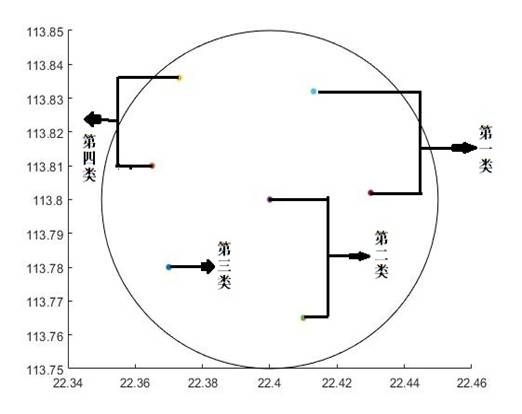
\includegraphics[width=7cm]{9.jpg}

3)价格的调整
根据以上的叙述,下面给出,价格微调的标准:1.对于失败的任务,如果$d_{i}>0$,则将其与$b_{\uppercase\expandafter{\romannumeral1}i}$相比较,如果$<b_{\uppercase\expandafter{\romannumeral1}i}$,则提升价格使之达到阈值,如果$>b_{\uppercase\expandafter{\romannumeral1}i}$,则不作调整;如果$d_{i}<0$;则将其与$b_{\uppercase\expandafter{\romannumeral3}i}$ 相比较,如果$<b_{\uppercase\expandafter{\romannumeral3}i}$,则提升价格使之达到阈值,如果>$b_{\uppercase\expandafter{\romannumeral3}i}$,则不作调整。2.对于成功的任务,如果$d_{i}>0$,则将其与$b_{\uppercase\expandafter{\romannumeral1}i}$ 相比较,如果<$b_{\uppercase\expandafter{\romannumeral1}i}$,则不作调整,如果>$b_{\uppercase\expandafter{\romannumeral1}i}$,降低价格使之达到阈值;如果$d_{i}<0$,则将其与$b_{\uppercase\expandafter{\romannumeral3}i}$ 相比较,如果<$b_{\uppercase\expandafter{\romannumeral3}i}$,则不作调整,如果>$b_{\uppercase\expandafter{\romannumeral3}i}$,降低价格使之达到阈值。例如:

\newpage
\begin{table}[!h]\center\scriptsize
\begin{tabular}{|l|l|l|l|l|l|}
\hline

任务号码&	任务gps 纬度	&任务gps经度&	任务标价&	任务执行情况&	调整之后的价格\\
\hline
{\color{red}{A0001}}&	{\color{red}{22.56614225}}&	{\color{red}{113.9808368}}&{\color{red}{66}}	&{\color{red}{0}}	&{\color{red}{68.362}}\\
\hline
{\color{red}{A0002}}&	{\color{red}{22.68620526}}&	{\color{red}{113.940525 2}}&	{\color{red}{65.5}}&	0&	{\color{red}{69.424}}\\
\hline
{\color{blue}{A0003}}&	{\color{blue}{22.57651183}}&	{\color{blue}{113.957198}}&	{\color{blue}{65.5}}	&{\color{blue}{1}}	&{\color{blue}{64.809}}\\
\hline
{\color{green}{A0004}}&	{\color{green}{22.56484081}}&	{\color{green}{114.2445711}}&	{\color{green}{75}}	&{\color{green}{0	}}&{\color{green}{75}}\\
\hline
{\color{red}{A0005}}&	{\color{red}{22.55888775}}&	{\color{red}{113.9507227}}&	{\color{red}{65.5}}&	{\color{red}{0}}&{\color{red}{67.771}}\\
\hline
{\color{green}{A0006}}&{\color{green}{22.55899906}}&	{\color{green}{114.2413174}}&	{\color{green}{75	}}&{\color{green}{0}}	&{\color{green}{75}}\\
\hline
{\color{green}{A0007}}&{\color{green}{22.54900371}}&	{\color{green}{113.9722597}}	&{\color{green}{65.5}}	&{\color{green}{1}}	&{\color{green}{65.5}}\\
\hline
{\color{red}{A0008}}&	{\color{red}{22.56277351}}&	{\color{red}{113.9565735}}	&{\color{red}{65.5	}}&{\color{red}{0	}}&{\color{red}{66.716}}\\
\hline
{\color{red}{A0009}}&	{\color{red}{22.50001192}}&{\color{red}{113.8956606	}}	&{\color{red}{66}}	&{\color{red}{0}}	&{\color{red}{69.065}}\\
\hline
\color{blue}{A0010}&	{\color{blue}{22.5437861}}&	{\color{blue}{113.9239778}}&{\color{blue}{66}}	&{\color{blue}{1}}	&{\color{blue}{65.711}}\\
\hline
{\color{red}{A0011}}&	{\color{red}{22.52486369	}}&{\color{red}{113.9308596}}&	{\color{red}{65.5	}}&{\color{red}{0}}&	{\color{red}{67.713}}\\
\hline
{\color{red}{A0012}}&	\color{red}{22.519087}&{\color{red}{113.9358436}}&{\color{red}{	65.5}}	&{\color{red}{0}}&	{\color{red}{68.416}}\\
\hline
{\color{green}{A0013}}&	{\color{green}{22.54797243}}&{\color{green}{113.977909}}&	{\color{green}{65.5}}	&{\color{green}{1}}&{\color{green}{65.5}}\\
\hline


\end{tabular}
\end{table}


图中价格提升的标记为蓝色,价格下降的标记为红色,价格不作调整的标记为绿色。

从表格中还能获取以下的信息:

1.重新定价的任务数占总任务数的60\%,也即绝大多数任务将被重新定价,由此可知模型对绝大多数任务有效,可见模型的合理性;

2.在价格未作调整的任务中,原先未完成的任务只有65个,占总任务数的8\%。这些任务可视为价格调整过后无法被完成的任务。所以可知,价格调整过后,任务完成率将达到92\%,由此可见模型的优越性。

3.经过统计可知,提升价格所需的资金为652元,而多出的价格只有289,之间的落差是APP平台需要补入的资金。

优缺点分析:
	
优点:能够给出一个阈值标准,定量精准的判断价格变化之后任务的执行情况;

缺点:只是在原有的基础上对价格进行微小的调整,没能从根本上提出更为优越的定价方案。

\

\textbf{角度二:}优化问题一中的线性模型
    对问题一,我们采用的线性模型中,将会员的预选限额,预选时间以及信誉度当成独立的变量,但是在题目当中指出,信誉度越高,预选时间越长,预选限额也越大,所以我们在优化问题一中的模型时,可以考虑这三个量之间的相互关系,重新定价,具体做法如下

1)模型的优化

原先的模型是

$v^{l}_{i}=a^{j}|r^{j}_{i}-\overline{r^{j}}|+a^{w}|r^{w}_{i}-\overline{r^{w}}|$
$+\sum\limits_{k\in O}(q^{j}|h^{j}_{k}-\overline{h^{j}}|+q^{w}|h^{w}_{k}-\overline{h^{w}}|+x_{k}(p_{3}((h^{j}_{k}-r^{j}_{i})^{2}+(h^{w}_{k}-r^{w}_{i})^{2})^{\frac{1}{2}}+p_{1}t_{k}+p_{2}e_{k})+c$

现在加入$x_{i}$对$e_{i}$和$t_{i}$的影响之后,模型变为

$v^{l}_{i}=a^{j}|r^{j}_{i}-\overline{r^{j}}|+a^{w}|r^{w}_{i}-\overline{r^{w}}|$
$+\sum\limits_{k\in O}(q^{j}|h^{j}_{k}-\overline{h^{j}}|+q^{w}|h^{w}_{k}-\overline{h^{w}}|+x_{k}(p_{3}((h^{j}_{k}-r^{j}_{i})^{2}+(h^{w}_{k}-r^{w}_{i})^{2})^{\frac{1}{2}}+p_{1}(t_{k}+n_{1}x_{k})+p_{2}(e_{k}+n_{2}x_{k}))+c$

因此我们的目标变为是找到一组系数$a^{j}$,$a^{w}$,$q^{j}$,$q^{w}$,$p_{3}$,$p_{1}$,$p_{2}$ ,$n_{1}$,$n_{2}$,$c$,使得
$ \sum\limits^{n}_{k=1}|v^{s}_{k}-v^{l}_{k}|$
达到最小。

2)重新拟合

和问题一中的做法一样,使用线性回归,但是会发现,现有的方程不足以解出$n_{1}$,$n_{2}$,所以,我们保证$n_{1}^{2}+n_{2}^{2}$达到最小,最后求解得到

 \ \ \ \ \ \ \  \ \ \  \ \ \ \ \ \ \  \ \ \  \ \ \ \ \ \ \  \ \ \ $ n_{1}=0$ \ \ \ \ \ \ \  \ \ \   $ n_{2}=   0.00335$

这说明,$x_{i}$对$e_{i}$有正向的影响,而对于$t_{i}$无影响。和题目中所说的基本吻合。


并且重新拟合之后,会发现新的理论价格和原始的理论价格有不同。

  \begin{table}[!h]\center\scriptsize
\begin{tabular}{|c|c|c|c|c|c|c|}
\hline

任务号码&	任务gps 纬度	&任务gps经度&	任务标价	&任务执行情况	&原始理论价格&	新的理论价格\\
\hline
A0001&	22.56614225&	113.9808368	&66	&0	&67.139	&66.862\\
\hline
A0002&	22.68620526&	113.9405252	&65.5	&0&	68.678&	68.864\\
\hline
A0003&	22.57651183&	113.957198	&65.5	&1&	65.117&	64.791\\
\hline
A0004&	22.56484081&	114.2445711	&75	&0&	68.629&	68.779\\
\hline
A0005&	22.55888775&	113.9507227	&65.5	&0	&67.12	&65.497\\
\hline
A0006&	22.55899906&	114.2413174	&75	&0	&68.68	&68.787\\
\hline
A0007&	22.54900371&	113.9722597	&65.5	&1	&67.342	&66.07\\
\hline
A0008&	22.56277351&	113.9565735	&65.5	&0	&65.845	&64.222\\
\hline
A0009&	22.50001192&	113.8956606	&66	&0	&68.314	&68.465\\
\hline
A0010&	22.5437861&	113.9239778	&66	&1	&68.091	&67.934\\
\hline
A0011&	22.52486369&	113.9308596	&65.5&	0	&68.24&	68.321\\
\hline
A0012&	22.519087	&113.9358436	&65.5&	0	&68.204	&68.249\\
\hline
A0013&	22.54797243&	113.977909	&65.5&	1	&67.621&	66.185\\
\hline
A0014&	22.50616871&	113.9314284	&66	&1	&68.216	&68.268\\
\hline
A0015&	22.49962566	&113.9365145	&66&	1	&68.221	&68.271\\
\hline
A0016&	22.54032142	&113.9236456	&66	&1&	68.167	&68.149\\
\hline




\end{tabular}
\end{table}


3)根据新的模型重新计算增值比

根据新的理论价格,我们可以重新计算增值比,然后沿用上述的理论,重新计算阈值,然后对价格进行微调。这里不再赘述,只附上新的增值比。
\newpage
  \begin{table}[!h]\center\scriptsize
\begin{tabular}{|c|c|c|c|c|c|c|}

\hline
任务号码&	任务gps 纬度&	任务gps经度	&任务标价	&任务执行情况&	原始增值比	&新的增值比\\
\hline
A0001&	22.56614225	&113.9808368	&66	&0	&-0.016962&	-0.012899\\
\hline
A0002&	22.68620526	&113.9405252	&65.5&	0&	-0.046274	&-0.048845\\
\hline
A0003&	22.57651183	&113.957198	&65.5	&1&	0.0058834	&0.010948\\
\hline
A0004&	22.56484081	&114.2445711	&75	&0&	0.092828	&0.090443\\
\hline
A0005&	22.55888775	&113.9507227	&65.5&	0	&-0.024142	&0.0000513\\
\hline
A0006&	22.55899906	&114.2413174	&75	&0&	0.092014&	0.090328\\
\hline
A0007&	22.54900371	&113.9722597	&65.5&	1&	-0.027352&	-0.008623\\
\hline
A0008&	22.56277351	&113.9565735	&65.5&	0&	-0.0052464&	0.019906\\
\hline
A0009&	22.50001192	&113.8956606	&66	&0&	-0.033875&	-0.036005\\
\hline
A0010&	22.5437861	&113.9239778	&66	&1&	-0.030706&	-0.028466\\
\hline
A0011&	22.52486369	&113.9308596	&65.5	&0&	-0.040156	&-0.041295\\
\hline
A0012&  22.519087	&113.9358436	&65.5&	0&	-0.039639&	-0.040285\\
\hline
A0013&	22.54797243	&113.977909	&65.5	&1&	-0.03136	&-0.010349\\
\hline
A0014&	22.50616871	&113.9314284	&66	&1&	-0.03249	&-0.033222\\
\hline
A0015&	22.49962566	&113.9365145	&66	&1&	-0.032557	&-0.033267\\
\hline
A0016&	22.54032142	&113.9236456	&66	&1&	-0.031787	&-0.031538\\
\hline




\end{tabular}
\end{table}


 优缺点分析:

优点:优化了原有的模型,沿用了上述的方法。

缺点:只是在原有的基础上对价格进行微小的调整,没能从根本上提出更为优越的定价方案。



\textbf{角度三:}线性规划选择最优系数

根据上述的讨论可知,我们假设定价模型是一个线性模型,最终的定价取决于系数的选择。并且由表一的数据我们知道,在实际的定价下,并不是所有的任务都完成,所以实际给出的价格不能作为阈值价格,只能作为阈值价格一个限界。所以我们做出如下假设:对于任务$i$,当任务完成时,认为理论价格$v^{l}_{i}$<实际价格$v^{s}_{i}$;当任务失败时,认为理论价格$v^{l}_{i}>$ 实际价格$v^{s}_{i}$.例如:

对第833个任务

\begin{table}[!h]\scriptsize\centering
 \begin{tabular}{|c|c|c|c|c|c|}
 \hline
 任务号码&任务GPS纬度&任务GPS经度&任务标价&任务执行情况&原始增值比\\
 \hline
 A0833&22.81467597&113.8277312&85&1&0.23214\\
 \hline
 \end{tabular}
 \end{table}
  有

  $v^{l}_{833}=a^{j}|r^{j}_{833}-\overline{r^{j}}|+a^{w}|r^{w}_{833}-\overline{r^{w}}|$
$+\sum\limits_{k\in O}(q^{j}|h^{j}_{k}-\overline{h^{j}}|+q^{w}|h^{w}_{k}-\overline{h^{w}}|+x_{k}(p_{3}((h^{j}_{k}-r^{j}_{833})^{2}+(h^{w}_{k}-r^{w}_{833})^{2})^{\frac{1}{2}}+p_{1}t_{k}+p_{2}e_{k})+c $
$\leq 85$

 对第101个任务
 \begin{table}[!h]\scriptsize\centering
 \begin{tabular}{|c|c|c|c|c|c|}
 \hline
 任务号码&任务GPS纬度&任务GPS经度&任务标价&任务执行情况&原始增值比\\
 \hline
 A0101&22.73006657&114.0666477&66.5&0&-0.034279\\
 \hline
 \end{tabular}
 \end{table}

 有

 $v^{l}_{101}=a^{j}|r^{j}_{101}-\overline{r^{j}}|+a^{w}|r^{w}_{101}-\overline{r^{w}}|$
$+\sum\limits_{k\in O}(q^{j}|h^{j}_{k}-\overline{h^{j}}|+q^{w}|h^{w}_{k}-\overline{h^{w}}|+x_{k}(p_{3}((h^{j}_{k}-r^{j}_{101})^{2}+(h^{w}_{k}-r^{w}_{101})^{2})^{\frac{1}{2}}+p_{1}t_{k}+p_{2}e_{k})+c $
$\geq 66$

这样可以得到800多个不等式,可以使用线性规划[3]中的单纯形法,求解出最优解。但是此时一个比较关键的问题是,我们无法找到一个阈值,从而很难判断在系数最优解的情况下,这些任务完成与否。所以该方法仅做参考。

优缺点分析:

优点:另辟蹊径,从根本上优化了定价模型

缺点:算法运行效率低,难以求解,并且缺少进一步的理论确定出新的阈值来判断任务执行情况。

\subsection{问题3分析}
问题3中提到,由于一些任务位置较为集中,会员争相竞争,从而导致一些任务
无人问津。这个现象可以从问题2中的优化角度一,利用增值比定量地看出。以任务$i$为例,任务$i$的实际价格比理论价格要高,即$d_{i}>0$,但是相比于周边的任务,增值比$d_{i}$ 较小,所以,任务$i$无人问津,任务失败。



 \ \ \ \ \ \ \  \ \ \  \ \ \ \ \ \ \  \ \ \  \ 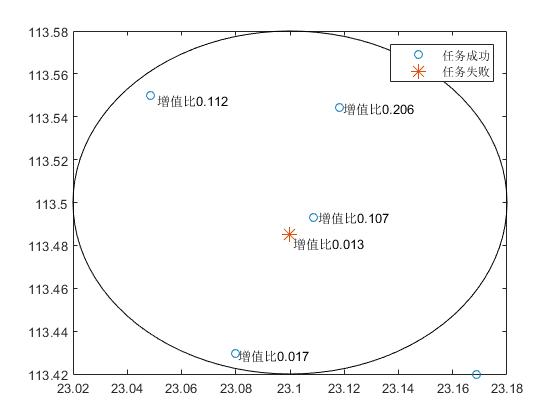
\includegraphics[width=7cm]{12.5.jpg}

问题出现的根本原因是,在任务密集的区域,由于竞争激烈,增值比上的微小差异被放大,最终给任务的完成与否带来的决定性的影响。想要解决这个矛盾,很自然的想法是把位置邻近,增值比相近的任务打包处理,用整体的增值比代替单个的增值比,这样能消除任务之间增值比上的微小差异,从而避免竞争带来的不利影响。

但是在具体提出打包分类方案时,我们会面临以下的难题:

1.每个任务包中包含多少任务最宜;

2.对任务进行聚合分类时,优先顺序该如何确定;

3.具体的分类标准是什么。

下面我们就逐步回答上述问题,提出我们的打包分类方案:

\textbf{Step 1:每个任务包中包含多少任务最宜}

每个任务包中任务数的多少对于分类模型最终的效果有着决定性的的影响:如果任务包中任务数过多,则由于会员预定限额的限制,选取这个任务包的会员就会很少,因此对任务包而言,选择执行会员的空间减少。并且任务过多,毫无疑问会降低任务完成的效率;而如果任务数过少,则体现不出打包分派任务的优越性。因此我们必须合理选择任务包中的任务数。通过分析附件二中的数据,从会员的预定限额可以看出,如果将所有的任务都打包处理,则对于一些任务预定限额很少的会员,将没有机会领取任务,这是人力资源的浪费,所以我们没有必要对所有任务都打包处理。通过上面的分析,可以综述如下:对于任务包中的任务数,我们需要找到一个上限。通过权衡,我们决定选取平均竞争任务数$m_{r}$=会员预定总限额/会员总数,作为包裹中任务数的上限。$m_{r}$在前文已经使用过,但是在这里$m_{r}$的含义略有不同,解释为平均每个会员能够领取到多少个任务,由上文的计算可知,$m_{r}=7$.

\textbf{Step 2: 打包优先顺序的决定}

任务打包的优先顺序与任务的位置分布息息相关。再次观察任务分布图,结合拓扑学和离散数学的知识[4],我们可以将任务分布形成的集合近似成一个单连通的区域。
即此时区域是连通的,且内部没有空洞,边界只有外围的一圈。

如果我们从内部开始分类打包,则会出现如下的情形:每次打包完一个任务包,就等于在原来的区域内部挖去一块,留下一个空洞,并且新增了一圈边界。如图:

 \ \ \ \ \ \ \  \ \ \  \ \ \ \ \ \ \  \ \ \  \  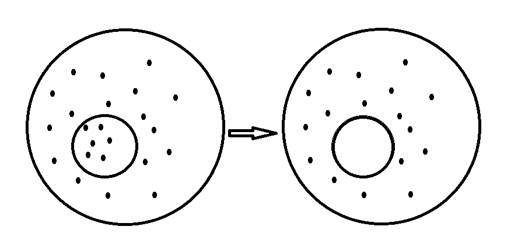
\includegraphics[width=10cm]{13.jpg}

 空洞的出现破坏了原来区域的单连通性,当空洞数目过多,原来的区域则被分割成互不相交的几块,这种情形不仅给算法的实现带来了巨大的困难,而且对于在分割出的区域内的任务,可能无法再使用之前的打包分类原则进行打包。如图:

  \ \ \ \ \ \ \  \ \ \  \ \ \ \ \ \ \  \ \ \  \ 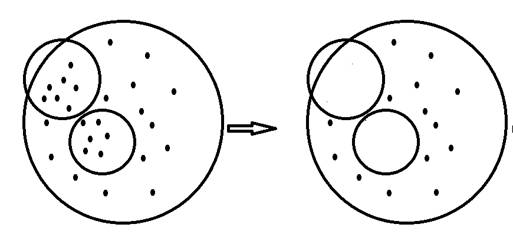
\includegraphics[width=10cm]{14.jpg}

 此外,对于新增边界处的任务,对它们进行打包也有不小的困难,如图:

\begin{figure}\center
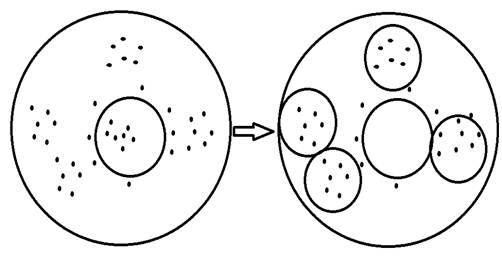
\includegraphics[width=10cm]{15.jpg}
\end{figure}

  基于以上的考虑,我们决定采用从外围开始打包的策略[5]。

\textbf{Step 3:具体打包方案}


重心转移法

\textbf{算法思路:}

根据step2,我们采取从外围开始打包的策略。更具体地讲,我们选择从离重心最远的那个点着手。因此,首先求出整个任务分布位置的重心,然后计算距离,求出距离重心最远的那个任务。接下来以这个任务为中心,在这里我们设置了一个最大距离l,以l为半径画圆,如果圆圈内的任务数不超过7,则将圈内的任务打包;如果圆圈内的任务超过7,则减小半径,使得圈内的任务数小于7为止。选取完毕后,将圈内的任务视为一个包裹。

 \ \ \ \ \ \ \  \ \ \  \ \ \ 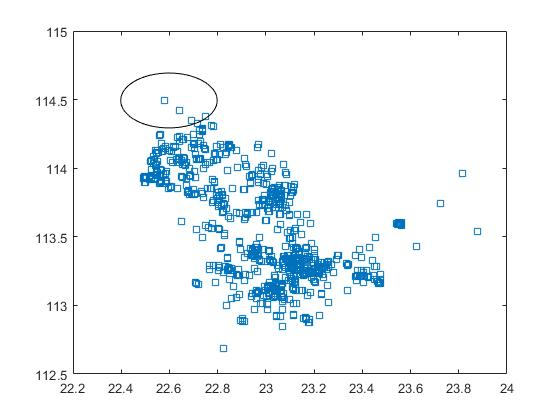
\includegraphics[width=10cm]{16.jpg}

  这时从整体的任务中除去这些已经打包的任务,得到一个新的集合,重新计算这个新的点集的重心位置,重复上述过程,便能将所有的任务进行分类打包.

打包结果,例如:

\begin{table}[!h]\center\scriptsize
\begin{tabular}{|c|c|c|c|}
\hline

包的编号	&包内的任务编号	&包的重心&	包的实际价格		\\
\hline
1	&A0450\  A0038\  A0063\  A0050	&22.638 114.421&	305	\\
\hline
80&	A0157\   A0210\   A0149\   A0148\   A0150\   A0182\   A0129	&23.138 113.458&	477.5		\\
\hline
100	&A0688 \  A0735\   A0550\   A0167\   A0788\   A0176\   A0553&	23.217 113.185	&507.5	\\
\hline

\end{tabular}
\end{table}


\textbf{进一步的拟合:}

将任务打包完成之后,我们建立新的线性回归模型来探索对任务完成的情况

(1)模型的建立

     以第i个任务包为例,在这个任务包中共有k个任务($k\leq 7$),我们利用数据聚合作如下的定义:

     $$V^{s}_{i}=\sum_{m\in O}v^{s}_{m}$$
     $$R^{j}_{i}=\frac{\sum_{m\in O}r^{j}_{m}}{k}$$
     $$R^{w}_{i}=\frac{\sum_{m\in O}r^{w}_{m}}{k}$$

     例如:

\begin{table}[!h]\center\scriptsize
\begin{tabular}{|c|c|c|c|c|}
\hline

包的编号	&包内的任务编号	&包的重心&	包的实际价格	&包的理论价格	\\
\hline
1	&A0450\  A0038\  A0063\  A0050	&22.638 114.421&	305	&285.114\\
\hline
80&	A0157\   A0210\   A0149\   A0148\   A0150\   A0182\   A0129	&23.138 113.458&	477.5	&474.413	\\
\hline
100	&A0688 \  A0735\   A0550\   A0167\   A0788\   A0176\   A0553&	23.217 113.185	&507.5	&487.26\\
\hline

\end{tabular}
\end{table}


 和问题一一样,假设$V^{s}_{i}$ 与变量$| R^{j}_{i} -\overline{r^{j}}|$,$|R^{w}_{i}-\overline{r^{w}}|$,$((h^{j}_{k}-r^{j}_{i})^{2}+(h^{w}_{k}-r^{w}_{i})^{2})^{\frac{1}{2}}$,$t_{m}$,$e_{m}$成线性关系
,模型的最终目的是确定出最优的一组系数$A^{j}$,$A^{w}$,$P_{1}$,$P_{2}$,$P_{3}$,$C$

(2)数学描述

$V^{l}_{i}=A^{j}|R^{j}_{i}-\overline{r^{j}}|+A^{w}|R^{w}_{i}-\overline{r^{w}}|$
$+\sum\limits_{k\in O}x_{m}(P_{3}((h^{j}_{m}-R^{j}_{i})^{2}+(h^{w}_{m}-R^{w}_{i})^{2})^{\frac{1}{2}}+P_{1}t_{m}+P_{2}e_{m})+C $
使得$ \sum\limits^{n}_{k=1}|V^{s}_{k}-V^{l}_{k}|$求和达到最小

(3)模型的求解

利用线性回归求的系数

\begin{center}
 $ A^{w}=-21.1547696388467$

 $  A^{j}=44.0379709381243  $

$P_{1}= -0.0815823312844 $

 $ P_{2}= 0.0005053407382$

 $P_{3}=-0.0001669136836$

   $C=827.2566024862618$
\end{center}

   下面对于所求的系数作出相应的解释:


与第一问中的系数相比,可以发现打包过后所有系数的值都得到增大,这和将整个包当成一个单位处理,实际价格和理论价格均增大的情况是相符的。通过进一步的研究发现$A^{w}$和$a^{w}$,$A^{j}$和$a^{j}$符号仍然相同,且相对大小基本不变,所以在打包过后不改变问题一所得出的定价规律。对于$P_{1}$和$p_{1}$,$P_{2}$和$p_{2}$,他们符号相同,且相对大小也基本不变,只有$P_{3}$ 符号改变但是$P_{3}$ 值相对很小,对结果的影响可以忽略不计,因此可以认为这组系数符合要求。



(4)对任务完成情况的影响

在上述基础上,我们对这个模型的数据作出如下分析。

打包处理过后,我们重新计算每个任务包的增值比,并用任务包的增值比来作为一个任务包能否被完成的评判依据。
例如:

\begin{table}[!h]\center\scriptsize
\begin{tabular}{|c|c|c|c|c|c|}
\hline

包的编号	&包内的任务编号	&包的重心&	包的实际价格	&包的理论价格	&包的增值比\\
\hline
1	&A0450\  A0038\  A0063\  A0050	&22.638 114.421&	305	&285.114&	0.07\\
\hline
80&	A0157\   A0210\   A0149\   A0148\   A0150\   A0182\   A0129	&23.138 113.458&	477.5	&474.413	&0.007\\
\hline
100	&A0688 \  A0735\   A0550\   A0167\   A0788\   A0176\   A0553&	23.217 113.185	&507.5	&487.26&	0.042\\
\hline

\end{tabular}
\end{table}




根据之前的分析,我们采用任务包的增值比来代替单个的增值比,是希望消除任务之间增值比上的微小差异,从而避免竞争带来的不利影响。但是注意到,任务包中的任务原先的完成情况可能是参差不齐的,而打包处理后,他们的完成情况将被绑定,要么同时被完成,要么同时失败。所以这时选取一个合适的阈值来判断一个任务包完成与否显得尤为重要。

经过尝试可知,如果我们仍然选取问题2中的阈值$b_{\uppercase\expandafter{\romannumeral1}}$,$b_{\uppercase\expandafter{\romannumeral3}}$作为评判标准,将任务包的增值比$D_{i}$直接与之比较,以此来判断任务完成情况,则会得到结果:46个任务包成功,57 个任务包失败。这个结果显然不是我们想要的。并且通过分析就能发现上述的判断方法有很大的弊端:因为当任务聚类成任务包后,虽然无法完成的任务的不利因素得到了稀释,但同时整个任务包的性能必定比包内原先就能被完成的任务的性能要低,如果仍然采用之前评判单个任务的评判标准,显然是不合理的。

我们采用如下的判断方法:我们计算每个任务包中任务增值比的平均值,将这个平均值与任务包的增值比相比较。如果任务包增值比$D_{i}>$这个平均值,则意味着在打包过后,总体的性能得到了提高,此时任务包被完成的可能性变大,因此我们将这个任务包视为成功。计算可得,打包过后,共有73个任务包被完成,51个任务包失败,

(5)结论

经过打包处理,消除了增值比在邻近任务之间的微小差异,避免了恶性竞争的出现。从算法结果来看打包过后任务完成率总体略有提高。但是,此模型仍然具有缺陷,最为关键的是缺少进一步的理论来确定阈值的选取,更为精确的判断任务的执行情况。

\newpage
\begin{figure}
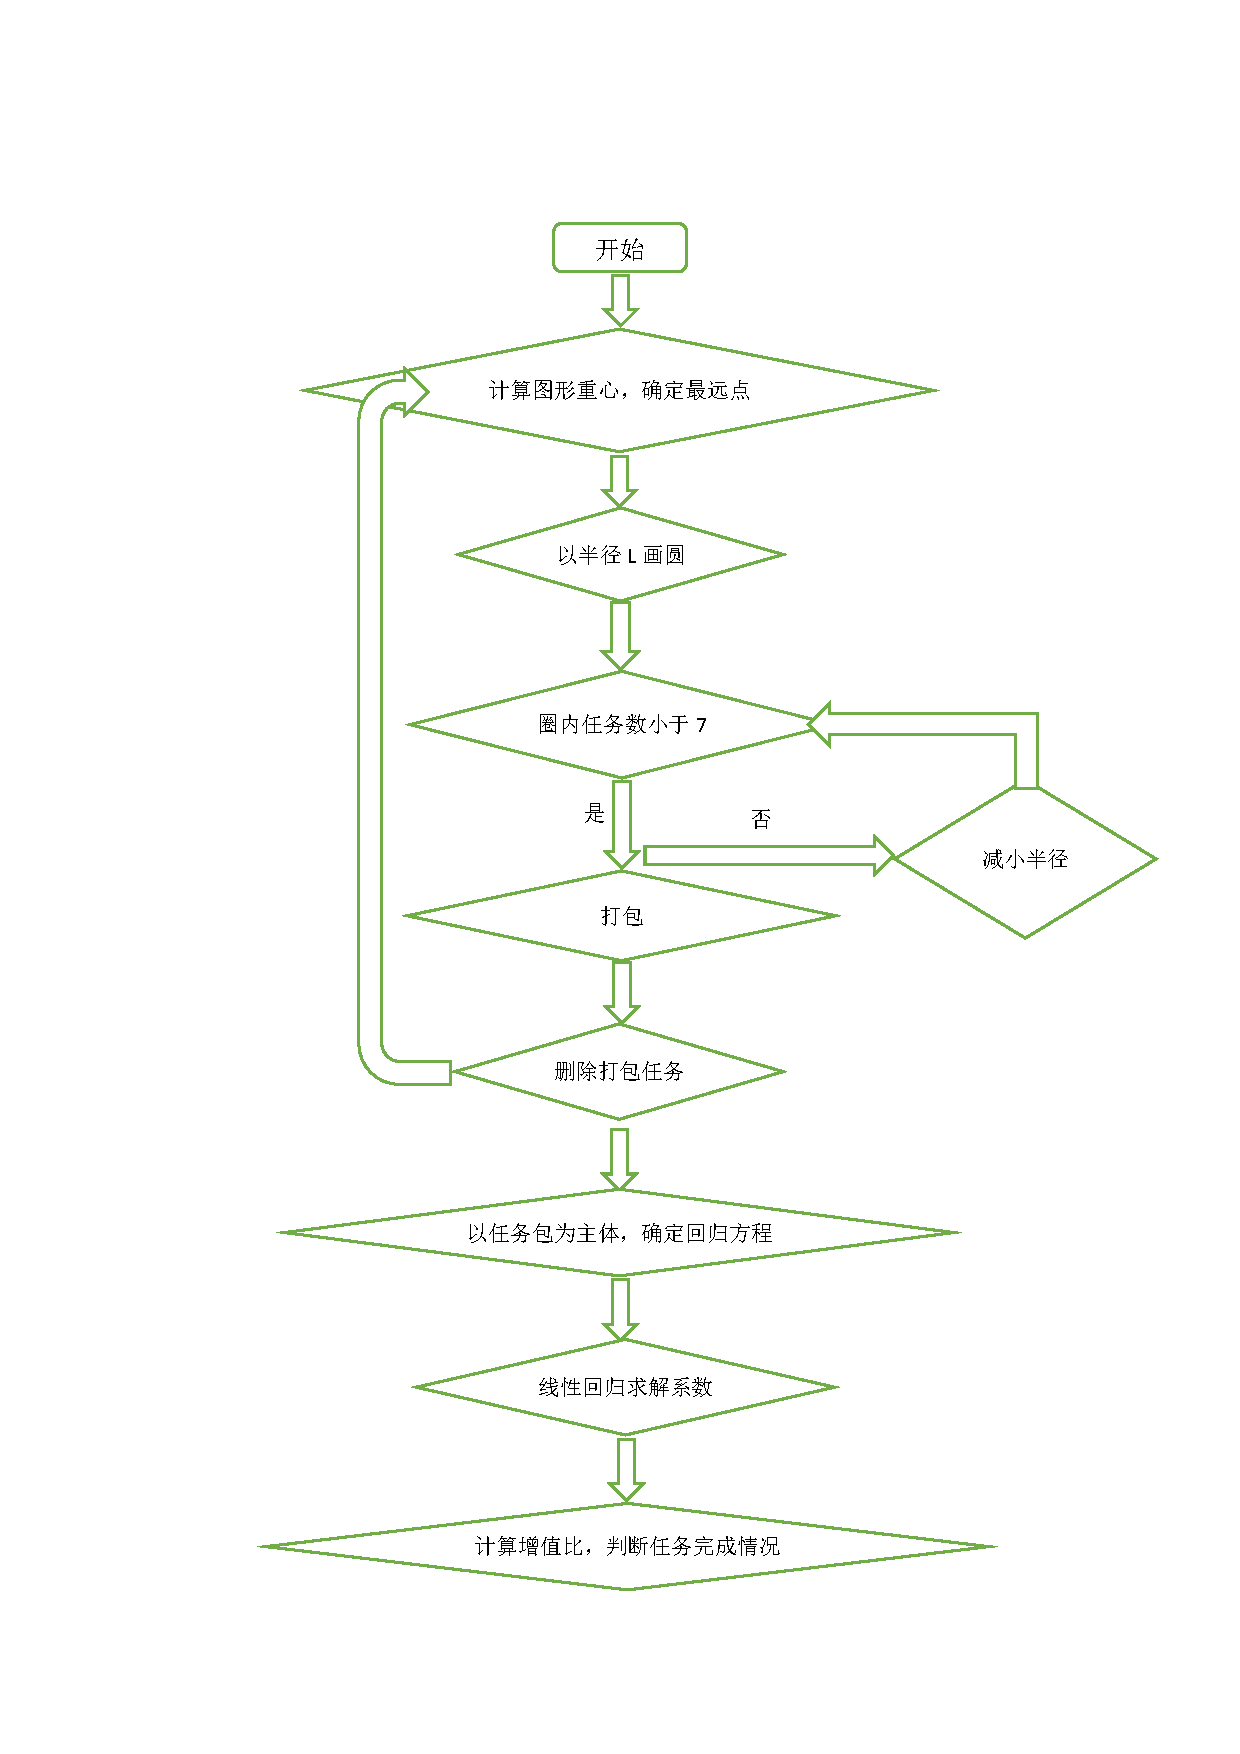
\includegraphics[width=9cm]{流程图3.pdf}\centering
\caption*{问题3流程图}
\end{figure}



\newpage
\subsection{问题4分析:}


从附件三我们可以看到,此次我们需要为两千多个任务定价。由前三问可知,我们可以选用问题一中的线性模型,为它们挨个定价,也可以采用问题三中的策略,先打包再对任务包定价。而此处,我们决定使用问题三中的策略,理由如下:

1.此次任务数目是原先的两倍多,竞争更为激烈,使用打包处理的策略能够避免恶性竞争,提高任务完成率。

2.此次会员需要执行的平均任务数增多,使用打包策略,能减少任务分配的时间,提高效率。

3.随着任务数的增多,问题一中的线性模型拟合匹配度降低,对于问题4可能不再适用。


因此,我们延继着前述的打包模型,先对任务打包,再利用前述的线性模型和求出的系数数据,可以得到每个包的定价。



例如

打包结果:

\begin{table}[!h]\centering\small
\begin{tabular}{|l|l|}
\hline
包的编号&	包的任务\\
\hline
1&	C1166\  C1146\  C1014\  C0011\  C0034\  C0039\  C0046	\\
\hline
150	&C1966\  C0891\  C1964\  C1965\  C1956\  C1962\  C0971	\\
\hline
300	&C0629	\\
\hline
\end{tabular}
\end{table}

定价方案:

\begin{table}[!h]\centering\small
\begin{tabular}{|l|l|l|}
\hline
包的编号&	包的任务&	包的价格\\
\hline
1&	C1166\  C1146\  C1014\  C0011\  C0034\  C0039\  C0046	&495.782\\
\hline
150	&C1966\  C0891\  C1964\  C1965\  C1956\  C1962\  C0971	&482.954\\
\hline
300	&C0629	&87.732\\
\hline
\end{tabular}
\end{table}


\section{\leftline{ 模型评估和改进}}
\subsection{ 模型的优点}
(1)选用线性模型探索定价规律,符合线性定价原则,基本探索出定价规律,为问题的后续深入奠定基础。

(2)采用外围收缩,重心转换的方法进行任务聚类,大大减小了计算复杂度,可操作性强。

\subsection{ 模型的缺点}
(1)未能充分利用数据信息,比如未能使用线性规划模型求解出最优的系数解,仍需对所给数据进一步挖掘。

(2)需要进一步改进任务聚类的方法,从外围收缩的算法是建立在将所有任务都打包的基础之上,在一些情况下,对于极端的边界点,可以选择剔除,在现有的模型中并没有给出这样的评判标准。

 \subsection{模型的改进和推广}
(1)改进:在已有的打包模型的基础上,可以只打包一部分任务点,对于剩下的任务点,用k近邻算法判断其所属的包。这避免了在判断较靠内部的点时,只由距离单个点的相对距离决定打包的缺陷。

(2)推广:在模型中添加非线性因素进行优化,使得模型可以考虑更多的因素。这样可以参考引用更多的数据,使得模型更加贴近现实。

\section*{参考文献}
[1] 罗荣华, 线性定价法则, 西南财经大学金融学院.

[2] 姜启源,谢金星,叶俊.数学模型[M]. 北京:高等教育出版社,2003.

[3] 张干宗.线性规划[M].武汉大学出版社,2010.

[4] 尤承业.基础拓扑学讲义[M].北京大学出版社,1997.

[5] 薛申芳.MATLAB在平面图形边界信息提取中的应用[J].衡水学院学报.2009.



\end{document}
















